\documentclass[conference]{IEEEtran}
\IEEEoverridecommandlockouts

% ==================== PREAMBLE ====================
% All \usepackage commands MUST be placed here, before \begin{document}
\usepackage{cite}
\usepackage{amsmath,amssymb,amsfonts}
\usepackage{algorithmic}
\usepackage{graphicx}
\usepackage{textcomp}
\usepackage{xcolor}
\usepackage{booktabs}
\usepackage{multirow}

\graphicspath{{figures/}}

\def\BibTeX{{\rm B\kern-.05em{\sc i\kern-.025em b}\kern-.08em
    T\kern-.1667em\lower.7ex\hbox{E}\kern-.125emX}}

% ==================== DOCUMENT BODY ====================
\begin{document}

\title{Robust Traffic Sign Classification Under Varying Environmental Conditions: A Comparative Study of CNN Architectures}

\author{\IEEEauthorblockN{1\textsuperscript{st} Awwab Wadekar}
\IEEEauthorblockA{\textit{Dept. of Computer Engineering and Information Technology} \\
\textit{Veermata Jijabai Technological Institute (VJTI)}\\
Mumbai, India \\
aswadekar\_b24@it.vjti.ac.in}
\and
\IEEEauthorblockN{2\textsuperscript{nd} Taha Valiji}
\IEEEauthorblockA{\textit{Dept. of Computer Engineering and Information Technology} \\
\textit{Veermata Jijabai Technological Institute (VJTI)}\\
Mumbai, India \\
tmvaliji\_b24@it.vjti.ac.in}
\and
\IEEEauthorblockN{3\textsuperscript{rd} Aditya Shimoga}
\IEEEauthorblockA{\textit{Dept. of Computer Engineering and Information Technology} \\
\textit{Veermata Jijabai Technological Institute (VJTI)}\\
Mumbai, India \\
ahshimoga\_b24@it.vjti.ac.in}
}

\maketitle

\begin{abstract}
Automated Traffic Sign Recognition (TSR) is essential for autonomous driving and advanced driver-assistance systems. However, environmental corruptions such as fog, snow, blur, and sensor noise can drastically reduce classification reliability. This paper evaluates the robustness of four Convolutional Neural Network (CNN) architectures -- a compact custom CNN (TrialCNN, 0.68M parameters), ResNet-18, MobileNetV2, and EfficientNet-B0 -- against 14 distinct environmental and digital corruption types across severity levels 1 to 5, following the corruption taxonomy of Hendrycks and Dietterich. All models are trained from scratch on three benchmark datasets -- GTSRB, BTSD, and CTSD -- using a grayscale preprocessing pipeline (median filtering with CLAHE contrast equalization) designed to suppress corruption-induced variance before it reaches the network. On clean test data, all four architectures exceed 88\% average accuracy, with TrialCNN reaching 96.9\%. Under the full corruption benchmark, however, the lightweight TrialCNN achieves the highest mean accuracy (79.5\%) and the smallest clean-to-corrupted accuracy gap (17.4 percentage points), outperforming the three substantially larger transfer-learning backbones; MobileNetV2 is the least robust, dropping 24.0 percentage points to a mean corrupted accuracy of 64.3\%. These results suggest that, for small, low-resolution traffic sign crops trained without ImageNet pretraining, model capacity and architectural depth do not translate into corruption robustness, and that preprocessing-level denoising is a more reliable lever than architecture choice alone.
\end{abstract}

\begin{IEEEkeywords}
Traffic Sign Recognition, Convolutional Neural Networks, Model Robustness, Image Corruptions, Deep Learning, Transfer Learning.
\end{IEEEkeywords}

\section{Introduction}
Autonomous vehicles rely heavily on vision-based traffic sign recognition to safely navigate complex environments. While Convolutional Neural Networks (CNNs) achieve high performance on standard, clean test benchmarks, their accuracy often degrades severely when exposed to real-world visual distortions.

In real-world deployment, images suffer from weather conditions (fog, snow, frost), capture artifacts (motion blur, defocus blur), and digital noise (Gaussian, shot noise, JPEG compression). Evaluating classification performance across controlled noise severities is vital to developing resilient deep-learning systems.

A natural question for practitioners is whether larger, ImageNet-style backbones are worth their additional computational cost when the end task is small-resolution sign recognition rather than general-purpose image classification. To probe this, we benchmark four architectures of increasing design sophistication -- a compact custom CNN, ResNet-18 \cite{resnet}, MobileNetV2 \cite{mobilenetv2}, and EfficientNet-B0 \cite{efficientnet} -- against 14 synthetic environmental corruptions across 5 severity levels, on three traffic sign datasets spanning different geographies and class counts. All models are trained from scratch (no ImageNet pretraining) on a common grayscale preprocessing pipeline, isolating the effect of architecture from the confound of pretrained feature reuse.

Our contributions are: (1) a unified robustness evaluation of four CNN architectures across three traffic sign benchmarks and 14 corruption types at 5 severities each (840 model--dataset--corruption--severity combinations in total); (2) an empirical finding that a small, non-pretrained CNN can match or exceed the corruption robustness of substantially larger transfer-learning backbones once a denoising preprocessing stage is applied; and (3) a preprocessing ablation showing the effect of a grayscale, median-filtered, CLAHE-equalized input pipeline relative to a naive resize-and-normalize baseline.

\section{Related Work}
Stallkamp et al. \cite{gtsrb} introduced the German Traffic Sign Recognition Benchmark (GTSRB) and showed that CNN-based classifiers can exceed human-level accuracy on clean, well-curated traffic sign images, establishing GTSRB as the de facto standard benchmark for the task. Subsequent work extended traffic sign recognition to other geographies and modalities: Zhang et al. \cite{ctsd} proposed a YOLOv2-based real-time detector for Chinese traffic signs and released an expanded Chinese Traffic Sign Dataset (CTSD), while the Belgium Traffic Sign Dataset (BTSD) has been widely used to study recognition under varied European road and lighting conditions. More recently, Sarwatt et al. \cite{btsd} studied the orthogonal problem of adversarial robustness in traffic sign classification, evaluating adversarial-example detection methods across Chinese, Belgian, and German traffic sign datasets and highlighting that robustness properties of TSR systems are highly dataset- and attack-dependent.

Separately from adversarial robustness, Hendrycks and Dietterich \cite{hendrycks2019robustness} proposed a standardized taxonomy of common, naturally occurring image corruptions (noise, blur, weather, and digital artifacts) at five severity levels, and showed that classification accuracy on ImageNet degrades substantially under these corruptions even when no adversary is present. We adopt this corruption taxonomy -- rather than adversarial perturbations -- because it better reflects the passive, non-malicious degradations (fog, motion blur, sensor noise, compression) that an onboard camera encounters during ordinary driving.

On the architecture side, He et al. \cite{resnet} introduced residual connections to enable training of substantially deeper CNNs, Sandler et al. \cite{mobilenetv2} introduced MobileNetV2's inverted residual and linear bottleneck design for efficient mobile inference, and Tan and Le \cite{efficientnet} introduced EfficientNet's compound scaling of depth, width, and resolution. All three are now standard choices for transfer learning in vision tasks, including prior traffic sign recognition pipelines; however, their relative corruption robustness when trained from scratch on small, low-resolution sign crops -- rather than fine-tuned from ImageNet weights on natural images -- has not been directly compared, which is the gap this paper addresses.

\section{Datasets and Noise Taxonomy}

\subsection{Benchmark Datasets}
Our experiments utilize three primary public traffic sign datasets, organized into the class splits used for training:
\begin{itemize}
    \item \textbf{German Traffic Sign Recognition Benchmark (GTSRB) \cite{gtsrb}:} 43 classes, 39{,}209 training and 12{,}630 test images.
    \item \textbf{Belgium Traffic Sign Dataset (BTSD):} 62 classes, 4{,}591 training and 2{,}534 test images, featuring varied lighting and real-world European road environments.
    \item \textbf{Chinese Traffic Sign Database (CTSD) \cite{ctsd}:} 58 classes, 4{,}931 training and 1{,}233 test images, captured under varied urban lighting conditions.
\end{itemize}
GTSRB is roughly an order of magnitude larger than BTSD and CTSD, which -- combined with its lower class count -- makes it a comparatively easier benchmark; BTSD, in contrast, combines the highest class count with the fewest training examples per class, and is consistently the most difficult dataset in our results (Section~\ref{sec:results}).

\subsection{Environmental Distortion Categories}
To rigorously evaluate model robustness, 14 visual corruptions from the Hendrycks and Dietterich taxonomy \cite{hendrycks2019robustness} are synthetically injected into the test sets at 5 discrete severity levels ($s \in \{1, 2, 3, 4, 5\}$), using the \texttt{imagecorruptions} reference implementation:
\begin{enumerate}
    \item \textbf{Noise Corruptions:} Gaussian Noise, Impulse Noise, Shot Noise.
    \item \textbf{Weather Corruptions:} Snow, Fog, Frost.
    \item \textbf{Blur Artifacts:} Motion Blur, Zoom Blur, Defocus Blur.
    \item \textbf{Digital \& Lighting Alterations:} Brightness, Contrast, Pixelate, Elastic Transform, JPEG Compression.
\end{enumerate}
Models are trained exclusively on clean (uncorrupted) data; corruptions are applied only at evaluation time, so reported degradation reflects generalization to unseen distortions rather than exposure during training.

\section{Methodology}

\subsection{Preprocessing Pipeline}
\label{sec:preproc}
Our preprocessing pipeline evolved over the course of the project. The initial baseline resized images to $32\times32$, converted them to RGB tensors, and applied channel-wise normalization with no denoising step. While simple, this pipeline left the network directly exposed to pixel-level noise and lighting artifacts, which we found contributed to disproportionately large accuracy drops under corruption.

We subsequently adopted a \emph{robust preprocessing shield} applied identically at training and evaluation time: each image is (1) resized to $32\times32$, (2) converted to grayscale, (3) denoised with a $3\times3$ median filter to suppress shot, impulse, and Gaussian pixel noise, and (4) contrast-equalized with Contrast-Limited Adaptive Histogram Equalization (CLAHE, clip limit 2.0, tile grid $4\times4$) to normalize fog-, brightness-, and contrast-type degradations. The output is converted to a single-channel float tensor and normalized to $[-1, 1]$. All architectures' first convolutional layer is adapted to accept a single input channel. All results reported in Section~\ref{sec:results} use this pipeline; we discuss the effect of the earlier RGB-only pipeline qualitatively in Section~\ref{sec:discussion}.

\subsection{Model Architectures}
We compare four CNN architectures, summarized in Table~\ref{tab:architectures}. None of the architectures use ImageNet-pretrained weights; all are trained from scratch so that differences in robustness reflect architectural inductive bias rather than pretrained feature reuse.
\begin{itemize}
    \item \textbf{TrialCNN} (custom baseline): a compact three-block CNN with $25 \to 50 \to 75$ channels, batch normalization, ReLU activations, max-pooling after each block, and a 512-unit fully connected head with dropout (0.2--0.3).
    \item \textbf{ResNet-18} \cite{resnet}: residual CNN with skip connections, adapted to single-channel input.
    \item \textbf{MobileNetV2} \cite{mobilenetv2}: depthwise-separable CNN using inverted residual bottlenecks, designed for efficient inference.
    \item \textbf{EfficientNet-B0} \cite{efficientnet}: compound-scaled CNN combining depthwise-separable MBConv blocks with squeeze-and-excitation attention.
\end{itemize}

\begin{table}[htbp]
\caption{Model Architectures and Parameter Counts (single-channel input, 43-class head)}
\begin{center}
\begin{tabular}{lcc}
\toprule
\textbf{Model} & \textbf{Parameters} & \textbf{Pretrained} \\
\midrule
TrialCNN         & 0.68M  & No \\
MobileNetV2      & 2.28M  & No \\
EfficientNet-B0  & 4.06M  & No \\
ResNet-18        & 11.19M & No \\
\bottomrule
\end{tabular}
\label{tab:architectures}
\end{center}
\end{table}

\subsection{Training Setup}
All models are trained independently per dataset for 100 epochs with the AdamW optimizer (learning rate $1\times10^{-3}$, weight decay $1\times10^{-4}$), a cosine-annealing learning-rate schedule, and mixed-precision (AMP) training with a batch size of 128. Because class distributions in all three datasets are imbalanced (particularly BTSD and CTSD), we use a class-balanced weighted cross-entropy loss, with weights computed from inverse class frequency on the training split. The checkpoint with the highest weighted test F1-score is retained for evaluation.

\subsection{Noise Robustness Evaluation Protocol}
For each trained model and dataset, we evaluate on the held-out test split corrupted by each of the 14 corruption types at each of the 5 severities independently (i.e., $14 \times 5 = 70$ corrupted test passes per model--dataset pair, $840$ in total across all four models and three datasets). For every corrupted test pass we record accuracy, weighted F1-score, precision, and recall, and we accumulate a confusion matrix aggregated across all corruptions and severities for qualitative error analysis.

\section{Results}
\label{sec:results}

\subsection{Baseline Performance (Clean Data)}
Table~\ref{tab:baseline_results} summarizes final-epoch test classification accuracy on uncorrupted data for all four architectures across the three datasets. All models achieve strong clean-data performance; TrialCNN and ResNet-18 are the strongest and most consistent, while MobileNetV2 is noticeably weaker on the data-scarce BTSD set. Weighted F1-scores track accuracy within 0.5 percentage points throughout and are omitted from the table for brevity.

\begin{table}[htbp]
\caption{Baseline Classification Accuracy (\%) on Uncorrupted Test Data}
\begin{center}
\begin{tabular}{lcccc}
\toprule
\textbf{Model} & \textbf{GTSRB} & \textbf{BTSD} & \textbf{CTSD} & \textbf{Avg.} \\
\midrule
TrialCNN         & 98.25 & 92.46 & 100.00 & 96.90 \\
ResNet-18        & 97.60 & 88.52 & 100.00 & 95.37 \\
EfficientNet-B0  & 97.70 & 80.27 & 99.27  & 92.41 \\
MobileNetV2      & 96.23 & 70.13 & 98.54  & 88.30 \\
\bottomrule
\end{tabular}
\label{tab:baseline_results}
\end{center}
\end{table}

\subsection{Robustness Under Environmental Degradation}
Table~\ref{tab:robust_results} reports mean accuracy for each model--dataset pair averaged over all 14 corruption types and 5 severity levels (70 corrupted evaluations per cell). Fig.~\ref{fig:clean_vs_corrupted} visualizes the clean-to-corrupted accuracy gap for each model, averaged across datasets.

\begin{table}[htbp]
\caption{Mean Accuracy (\%) Under Corruption, Averaged Over All 14 Corruption Types and 5 Severities}
\begin{center}
\begin{tabular}{lcccc}
\toprule
\textbf{Model} & \textbf{GTSRB} & \textbf{BTSD} & \textbf{CTSD} & \textbf{Avg.} \\
\midrule
TrialCNN         & 72.54 & 76.99 & 88.89 & 79.47 \\
ResNet-18        & 69.04 & 74.21 & 87.05 & 76.76 \\
EfficientNet-B0  & 75.00 & 65.36 & 83.21 & 74.53 \\
MobileNetV2      & 70.80 & 49.55 & 72.69 & 64.35 \\
\bottomrule
\end{tabular}
\label{tab:robust_results}
\end{center}
\end{table}

Despite having the lowest parameter count by over an order of magnitude (0.68M vs. 11.19M for ResNet-18), TrialCNN attains the \emph{highest} mean corrupted accuracy of all four architectures, and the smallest clean-to-corrupted drop (17.43 percentage points, vs. 18.61 for ResNet-18, 17.88 for EfficientNet-B0, and 23.95 for MobileNetV2). MobileNetV2 is the clear outlier: it is both the weakest model on clean data for two of the three datasets and the least robust under corruption, with its accuracy on BTSD falling to 49.55\% on average across corruptions -- close to chance for a 62-way classification task at the hardest severities.

Fig.~\ref{fig:severity_degradation} shows mean accuracy as a function of corruption severity, averaged across datasets and corruption types. TrialCNN and ResNet-18 degrade gradually and near-monotonically; EfficientNet-B0 and especially MobileNetV2 show larger, less consistent swings across severity levels, indicating higher sensitivity to specific corruption--severity combinations rather than uniform degradation.

\begin{figure}[htbp]
\centering
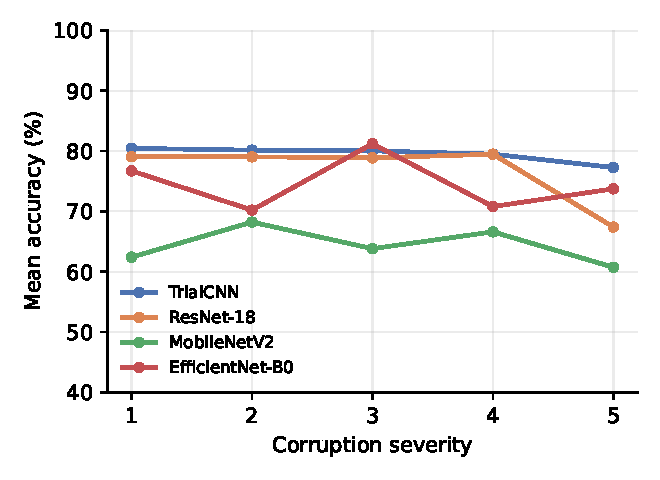
\includegraphics[width=0.95\linewidth]{severity_degradation.pdf}
\caption{Mean classification accuracy vs. corruption severity, averaged across all three datasets and 14 corruption types.}
\label{fig:severity_degradation}
\end{figure}

\begin{figure}[htbp]
\centering
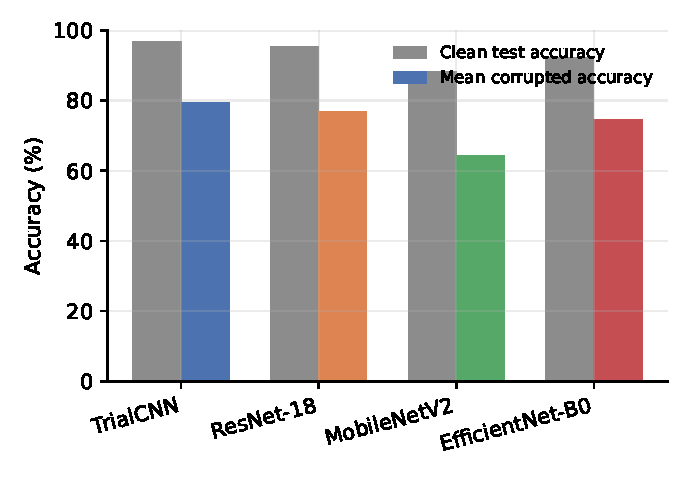
\includegraphics[width=0.95\linewidth]{clean_vs_corrupted.pdf}
\caption{Clean test accuracy vs. mean corrupted accuracy per model, averaged across the three datasets. The gap between bars reflects each architecture's robustness cost.}
\label{fig:clean_vs_corrupted}
\end{figure}

\subsection{Per-Corruption Breakdown}
Fig.~\ref{fig:corruption_heatmap} breaks mean accuracy down by individual corruption type and model (averaged across datasets and severities), sorted by TrialCNN's accuracy. Noise-type corruptions (impulse, shot, Gaussian) and weather corruptions (frost, fog) are generally handled well by TrialCNN and ResNet-18, consistent with the median-filtering and CLAHE stages of the preprocessing pipeline (Section~\ref{sec:preproc}) directly targeting these degradations. All four models find \emph{snow} and \emph{pixelate} among the more difficult corruptions, and MobileNetV2 is uniformly the weakest or near-weakest model across every corruption category, with \emph{zoom\_blur} (53.1\%) and \emph{impulse\_noise} (59.4\%) its hardest cases.

\begin{figure}[htbp]
\centering
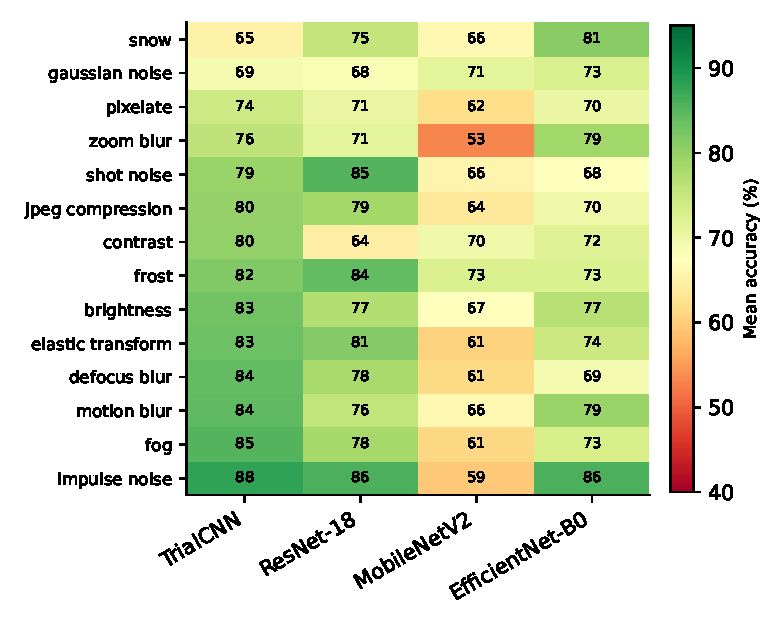
\includegraphics[width=\linewidth]{corruption_heatmap.pdf}
\caption{Mean accuracy (\%) by corruption type and model, averaged across the three datasets and 5 severity levels.}
\label{fig:corruption_heatmap}
\end{figure}

\subsection{Error Analysis}
Aggregating the per-model, per-dataset confusion matrices across all corruptions and severities shows that misclassifications are not spread uniformly across classes: for GTSRB in particular, a small cluster of visually similar sign classes accounts for a disproportionate share of all errors, while the majority of classes are rarely confused with one another even at high corruption severity. This suggests that further robustness gains may come less from global regularization and more from targeted augmentation or feature disambiguation for this small set of confusable classes; full per-class confusion matrices for every model--dataset pair are retained in the project's results directory for follow-up analysis.

\section{Discussion}
\label{sec:discussion}
The central empirical finding of this study is that, under our experimental conditions -- training from scratch, $32\times32$ single-channel inputs, and a denoising preprocessing stage -- larger and architecturally more sophisticated backbones do \emph{not} yield more corruption-robust classifiers. We offer three non-exclusive explanations. First, ResNet-18, MobileNetV2, and EfficientNet-B0 are designed and tuned for $224\times224$ three-channel ImageNet-scale inputs with pretrained initialization; at $32\times32$ resolution and without pretraining, their additional depth and stride structure may discard the fine spatial detail (such as the shape of a digit or pictogram) that distinguishes traffic sign classes, without the benefit of pretrained low-level filters to compensate. Second, the robust preprocessing shield already performs a substantial share of the denoising work before any image reaches the network, which likely narrows the advantage that deeper architectures would otherwise have in learning noise-invariant features end-to-end. Third, MobileNetV2's depthwise-separable convolutions, which trade representational capacity for efficiency, appear to be disproportionately sensitive to the pixel-level perturbations in our corruption suite, consistent with efficiency--robustness trade-offs reported for mobile-oriented architectures in the broader corruption-robustness literature \cite{hendrycks2019robustness}.

A secondary, more practical observation is that the earlier RGB resize-and-normalize pipeline used in initial project iterations produced visibly larger robustness gaps than the grayscale, median-filtered, CLAHE-equalized pipeline adopted for the results reported here, reinforcing that input-level preprocessing is a cheap and effective complement to (or substitute for) architectural capacity when robustness, not just clean accuracy, is the design goal.

\section{Limitations and Future Work}
This study has several limitations that bound the scope of our conclusions. First, all models are trained exclusively on clean data and never exposed to corrupted inputs during training; evaluating corruption-aware training strategies (e.g., mixed or probabilistic corruption augmentation, which our training pipeline already supports but was not used for the final models in this study) is a natural next step and may close the robustness gap for the deeper architectures. Second, our preprocessing shield converts inputs to grayscale, discarding color information that may be informative for some sign categories (e.g., red prohibition rings vs. blue mandatory signs); an ablation isolating the contribution of each shield component (median filtering vs. CLAHE vs. grayscale conversion alone) would clarify which stage drives the robustness improvement. Third, results are reported as accuracy and F1-score aggregated over severities and corruptions; a severity-stratified statistical significance analysis, and per-class robustness breakdowns beyond the aggregate confusion-matrix analysis in this paper, are left for the final version. Finally, all experiments use models trained from scratch; repeating the comparison with ImageNet-pretrained initialization would clarify whether the robustness advantage of the compact CNN is specific to the from-scratch, low-resolution regime studied here or persists more generally.

\section{Conclusion}
We presented a systematic robustness evaluation of four CNN architectures -- TrialCNN, ResNet-18, MobileNetV2, and EfficientNet-B0 -- trained from scratch on three traffic sign benchmarks (GTSRB, BTSD, CTSD) and evaluated against 14 environmental and digital corruptions at 5 severity levels each. While all four architectures achieve strong clean-data accuracy (88--97\% on average), the compact, 0.68M-parameter TrialCNN achieves both the highest mean accuracy under corruption (79.5\%) and the smallest robustness gap, outperforming all three substantially larger transfer-learning backbones; MobileNetV2 is consistently the least robust. Combined with the qualitative gains observed from our grayscale, median-filtered, CLAHE-equalized preprocessing pipeline relative to a naive RGB baseline, these results indicate that for small, low-resolution traffic sign recognition, careful preprocessing and a right-sized architecture are more effective levers for robustness than simply adopting a larger, more sophisticated backbone.

\section*{Acknowledgment}
We thank our project mentor for guidance throughout the evaluation and feedback process that shaped this study.

\begin{thebibliography}{00}
\bibitem{gtsrb} J. Stallkamp, M. Schlipsing, J. Salmen, and C. Igel, ``Man vs. computer: Benchmarking machine learning algorithms for traffic sign recognition,'' \textit{Neural Networks}, vol. 32, pp. 323--332, 2012.
\bibitem{hendrycks2019robustness} D. Hendrycks and T. Dietterich, ``Benchmarking neural network robustness to common corruptions and perturbations,'' in \textit{Proc. ICLR}, 2019.
\bibitem{ctsd} J. Zhang, M. Huang, X. Jin, and X. Li, ``A real-time Chinese traffic sign detection algorithm based on modified YOLOv2,'' \textit{Algorithms}, vol. 10, no. 4, p. 127, 2017.
\bibitem{btsd} D. S. Sarwatt, F. Kulwa, J. Ding, and H. Ning, ``Adapting image classification adversarial detection methods for traffic sign classification in autonomous vehicles: A comparative study,'' \textit{IEEE Transactions on Intelligent Transportation Systems}, 2024.
\bibitem{resnet} K. He, X. Zhang, S. Ren, and J. Sun, ``Deep residual learning for image recognition,'' in \textit{Proc. IEEE CVPR}, 2016, pp. 770--778.
\bibitem{mobilenetv2} M. Sandler, A. Howard, M. Zhu, A. Zhmoginov, and L.-C. Chen, ``MobileNetV2: Inverted residuals and linear bottlenecks,'' in \textit{Proc. IEEE CVPR}, 2018, pp. 4510--4520.
\bibitem{efficientnet} M. Tan and Q. Le, ``EfficientNet: Rethinking model scaling for convolutional neural networks,'' in \textit{Proc. ICML}, 2019, pp. 6105--6114.
\end{thebibliography}

\end{document}
